\chapter{Planificación}
En la vida real, a menudo pensamos en alcanzar una determinada meta, unos objetivos...
Metas y objetivos que por cuestiones externas, de logística o planificación no podemos
conseguir en el tiempo estimado o directamente conseguirlos. Por ejemplo, una simple
quedada con unos amigos, el tiempo dedicado a estudiar para un examen, realizar una
excursión... Todo ello requiere una organización y una planificación.\\

Lo anteriormente mencionado, se aplica exactamente igual para el desarrollo de
\textit{software}, si no se sigue una planificación rigurosa y exhaustiva, el desarrollo
puede no ser el esperado y puede no ser posible. En los siguientes puntos trataremos:

    \begin{enumerate}
        \item Metodología utilizada (\ref{sec:methodology}).
        \item Temporización (\ref{sec:timing}).
        \item Seguimiento del desarrollo(\ref{sec:tracking}).
    \end{enumerate}

\section{Metodología utilizada} \label{sec:methodology}
\subsection{Metodología ágil}
Para el desarrollo de este proyecto se ha seguido una \textbf{metodología ágil}
\cite{agile-methodology}, pero...¿qué son las metodologías ágiles? Pues bien, las
metodologías ágiles son aquellas que dividen el desarrollo de \textit{software} en pequeñas
piezas en funcionamiento (es decir, que cumplan su propósito), para poder hacer entregas
regulares al cliente y hacer que el desarrollo de \textit{software} sea flexible y productivo. Hay que tener
en cuenta que el desarrollo ágil no nos dice lo que hay que hacer en cada fase del
proyecto, sino que se trata de una guía para que el desarrollo de \textit{software} sea más
productivo y más eficiente. Por ejemplo, en los siguientes puntos:

    \begin{itemize}
        \item \textbf{Personas e interacciones} - Procesos y herramientas.
        \item \textbf{\textit{Software} en funcionamiento} - Documentación exhaustiva.
        \item \textbf{Respuesta ante cambios} - Plan definido.
    \end{itemize}

A pesar de estar relacionados los elementos de la izquierda (en negrita) con los de la
derecha, el desarrollo ágil nos sugiere que prestar más atención a los \textbf{puntos
de la izquierda} que a los de la derecha puede llevarnos a conseguir mejores resultados
en el desarrollo del \textit{software}.\\

Este desarrollo ágil ofrece una serie de ventajas \cite{advantages-agile-methodology}
destacadas:

    \begin{itemize}
        \item \textbf{Mayor objetividad} sobre el tiempo, costo o rendimiento que está
        teniendo el proyecto a lo largo del desarrollo.
        \item \textbf{Reducción de costes} gracias a la flexibilidad del desarrollo ágil.
        Los errores se van identificando y corrigiendo conforme se avanza en el proyecto.
        \item \textbf{Satisfacción del cliente} gracias a las entregas de producto
        periódicas que se van realizando, además de sentirse más involucrado con él.
        \item \textbf{Mejora continua} gracias al proceso iterativo que implica el desarrollo
        ágil. 
    \end{itemize}

Como se ha mencionado anteriormente, el desarrollo ágil no nos dice lo que hacer en cada fase
del desarrollo, entonces...¿quién nos lo dice? Es por ello que se ha procedido a usar un
marco ágil para el desarrollo como Scrum.\\

\subsubsection{Scrum} \label{subsubsec:scrum}
El marco de trabajo Scrum \cite{scrum} fue diseñado para equipos de trabajo de entre 5 y 9
personas, que en su conjunto forman el \textbf{equipo Scrum (\textit{Scrum Team})}, formado por los
\textbf{desarrolladores}, el \textbf{propietario del producto (\textit{Product Owner})} y el
\textbf{\textit{Scrum Master}}. Cada uno de ellos tiene una función concreta dentro del desarrollo
de \textit{software}, por lo que en este proyecto no tendría sentido utilizar Scrum al pie
de la, letra, ya que no existe un \textit{Product Owner}, ni un \textit{Scrum Master} supervisándolo todo. Sin
embargo, sí se han utilizado conceptos de este marco de trabajo como son los \textbf{\textit{sprints}}.\\.

El \textit{sprint} es el evento más importante de Scrum, donde las ideas se convierten en
valor para nuestra aplicación. Tiene una longitud fija de un mes como máximo de duración
(esta es la recomendación), pero lo habitual es que dure entre una y cuatro semanas. Cada
\textit{sprint} puede considerarse como un miniproyecto dentro del desarrollo y dentro de
este se suceden una serie de etapas:

    \begin{itemize}
        \item \textbf{Planificación de \textit{Sprint} (\textit{Sprint Planning})}: en esta fase se establece
        el trabajo a realizar en el \textit{sprint} y se responden las siguientes cuestiones:
            \begin{itemize}
                \item ¿Por qué es valioso el \textit{Sprint}?
                \item ¿Qué se puede hacer en el \textit{Sprint}?
                \item ¿Cómo se realizará el trabajo elegido?
            \end{itemize}
        \item \textbf{Scrum diario (\textit{Daily Scrum})}: en esta fase se inspecciona el progreso
        hacia la consecución del objetivo del \textit{sprint}. En este caso, dado que el
        proyecto se realiza por una persona, esta tendrá que hacer \textbf{autocríticas} y
        \textbf{autoevaluaciones}.
        \item \textbf{Revisión del \textit{Sprint} (\textit{Sprint Review})}: como su propio nombre indica,
        se revisa el trabajo realizado durante el \textit{sprint}. En este caso, sería
        revisado por el tutor académico o bien el arqueólogo, dando una retroalimentación al
        desarrollador.
        \item \textbf{La retrospectiva del \textit{Sprint} (\textit{Sprint Retrospective})}: finalmente, se
        hace una reunión para analizar cómo fue el \textit{sprint}, problemas que se encontraron,
        cómo fueron o no resueltos... todo ello con el equipo de Scrum. En este caso, al
        tratarse de un proyecto individual, hay que hacer dicho análisis individualmente. 
    \end{itemize}



% Cuando se empieza cada cosa
\section{Temporización} \label{sec:timing}
Para poder llevar a cabo un proyecto de \textit{software}, es necesario tener una idea de cuánto
tiempo se va a dedicar a cada uno de los pasos del desarrollo. En este caso, se ha
dedicado lo siguiente a cada uno de ellos:

\begin{table}[H]
        \centering
        \begin{tabular}{c c c } \hline
            \toprule
            \rowcolor{blue!50} 
            \textbf{Fases del desarrollo}   & \textbf{Fecha de inicio} & \textbf{Fecha de finalización} \\
            \midrule
            \rowcolor{blue!25} 
            Reuniones con el cliente        & 2 de febrero      & 7 de marzo    \\ 
            \rowcolor{blue!10} 
            Especificación de requisitos    & 2 de febrero      & 7 de marzo    \\ 
            \rowcolor{blue!25} 
            Planificación                   & 10 de febrero     & 15 de febrero \\ 
            \rowcolor{blue!10} 
            Elección de modelos             & 16 de febrero     & 8 de marzo \\ 
            \rowcolor{blue!25} 
            Implementación del \textit{software}     & 23 de febrero     & 11 de junio    \\ 
            \rowcolor{blue!10} 
            Documentación                   & 2 de febrero      & 25 de junio    \\ \bottomrule
        \end{tabular}
        \label{tab:planning}
        \caption{Tabla con la temporización del proyecto}
\end{table}

Como puede observarse, del 2 de febrero al 7 de marzo se han realizado las reuniones con
el cliente y simultáneamente se han ido obteniendo los requisitos necesarios que debe cumplir
el proyecto (requisitos funcionales, no funcionales y de información).\\

Posteriormente, del 10 al 15 de febrero, se comenzó a planificar el proyecto, es
decir, cómo se iba a proceder a trabajar, así como la forma de planificar y organizar dicho
trabajo. Esta planificación fue una especie de borrador para poder iniciar el proyecto, ya
que como puede observarse todavía se estaban manteniendo reuniones con el cliente.\\

Una vez hecha la planificación, se podía comenzar con la elección de modelos (del 16 de
febrero al 8 de marzo) para comenzar la implementación del proyecto, etapa que
tiene una duración de aproximadamente 4 meses (del 23 de febrero al 11 de junio).\\

La documentación es una de las partes más importantes del proyecto y como se puede observar,
se le ha dado el peso requerido, ya que esta se ha ido elaborando de forma progresiva desde
el inicio del proyecto hasta su finalización, dándole así una mayor calidad y rigor a la
documentación realizada.

% Github, git, reuniones con el tutor, etc.
\section{Seguimiento del desarrollo} \label{sec:tracking}
En esta sección se explica cómo se lleva a cabo el seguimiento del desarrollo del proyecto,
tanto desde el punto de vista del código como desde las reuniones que se van manteniendo
con el tutor académico \textbf{Daniel Sánchez Fernández}.\\

Desde el punto de vista del código, se ha decidido usar Github \cite{github}, un sitio web
que permite a millones de desarrolladores almacenar y administrar su código. Este hace uso,
como su propio nombre indica, de una herramienta de \textbf{control de versiones} llamada
Git \cite{git}, que permite el control de cambios en el código, así como de una herramienta
de gestión de código (GitHub) que permite almacenar los cambios realizados en el código.\\

Hablemos un poco de cómo funciona Git. Git es el sistema de control de versiones más
utilizado del mundo, es un proyecto de código abierto y creado por el famoso desarrollador
del kernel de Linux, \textbf{Linus Torvals}. Este sistema nos permite llevar un control de
cambios realizados en el código, de forma que podremos volver a estados pasados del mismo
a través de los \textbf{commits} (acción de guardar los archivos modificados en el
repositorio), además de tener más información de cada cambio como la hora de realización,
el autor del cambio, lo que se añadió, modificó o eliminó, etc. Además de todo esto, nos
permite crear \textbf{ramas (\textit{branches})}, que representan una línea independiente del
desarrollo, es decir, son copias de la versión principal del proyecto sobre las que podemos
trabajar sin afectar el código principal. Cabe destacar que existen muchas más
funcionalidades de Git que no se mencionarán, ya que no es el principal objetivo de este
apartado.\\

Por otra parte tenemos Github, que está completamente integrado con Git, ofreciéndonos una
interfaz gráfica genial donde podemos subir todo el proceso del proyecto en el repositorio
de Git y ver todos los commits, ramas, etc. que hemos ido creando, así como crearlos.
Además, nos ofrece muchas más funcionalidades que Git no nos ofrece, como la creación de
\textbf{\textit{issues}} (problemas), la creación de \textbf{\textit{pull requests}}
(solicitudes de cambios), creación de \textbf{repositorios} (repositorios de código),
herramientas para realizar \textbf{integración continua y distribución continua}, siendo
estas últimas explicadas en el \textit{sprint} correspondiente de la sección de
\textit{sprints} \ref{sec:sprints}, los \textbf{projects boards}, etc. Estos últimos se han
usado especialmente para realizar un seguimiento de las \textit{issues} que se van
completando en el proyecto, procedemos a explicar cómo.\\

Los \textbf{tableros de proyectos (project boards)} \cite{project-boards} son una
herramienta de Github que nos permite crear flujos de trabajo personalizados que se adapten
a las necesidades de nuestro proyecto, como el seguimiento y la priorización del trabajo de
características específicas. En este caso se ha utilizado para realizar un seguimiento
del estado en el que se encuentran las \textbf{\textit{issues}} que se van creando. Para
ello, se han definido las siguientes columnas:

    \begin{figure}[H]
        \centering
        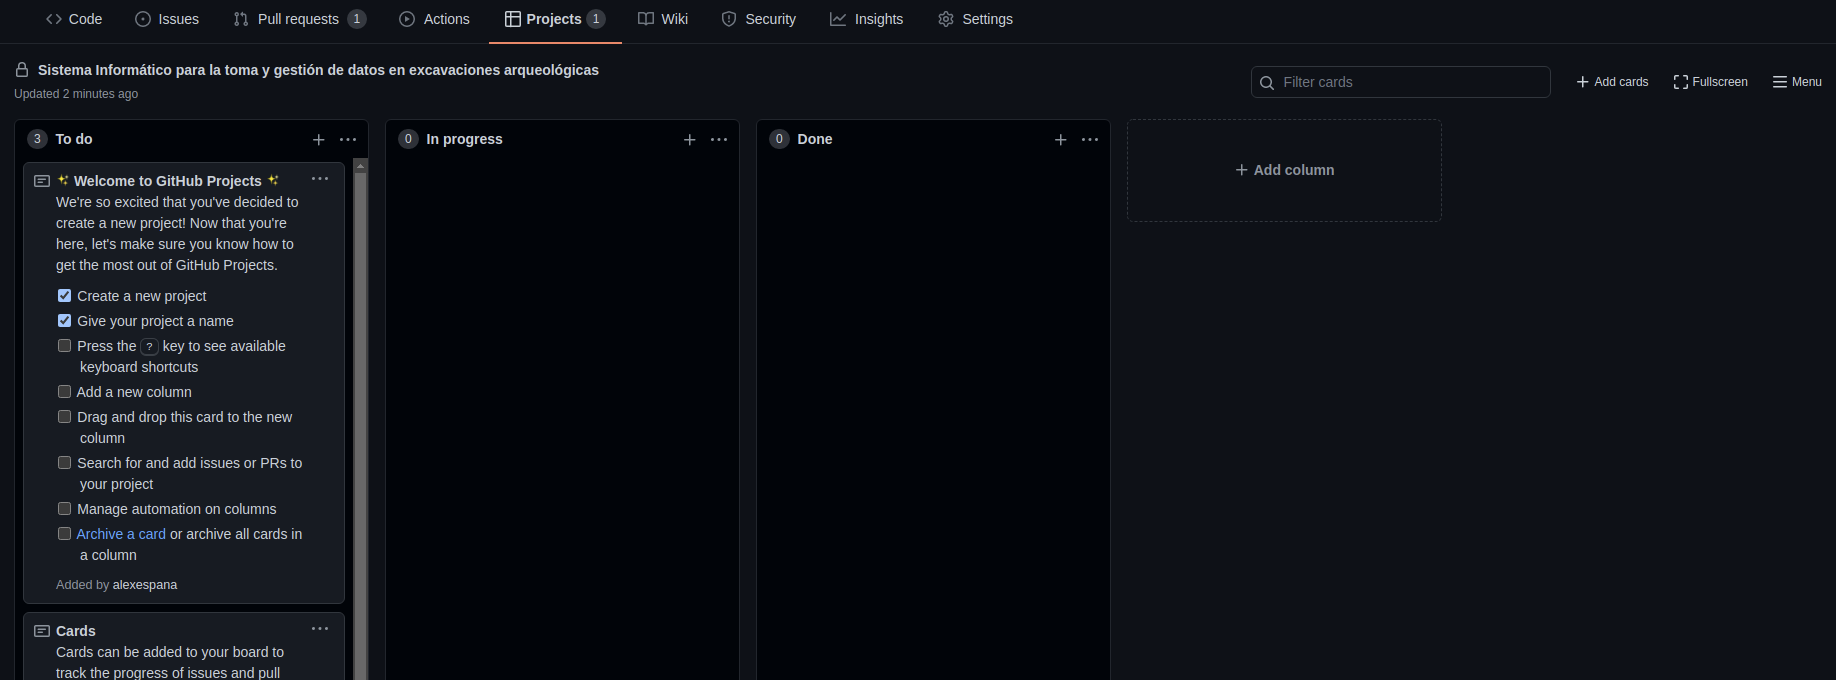
\includegraphics[scale=0.19]{imagenes/project-board.png}
        \caption[Tablero del proyecto]{Tablero del proyecto. Fuente \cite{project-board-image}}
        \label{fig:project-board}
    \end{figure}

    \begin{itemize}
        \item \textbf{\textit{To Do}}: corresponde a los \textit{issues} en los que no se ha
        empezado a desarrollar.
        \item \textbf{\textit{In Progress}}: corresponde a los \textit{issues} que se están
        desarrollando.
        \item \textbf{\textit{Done}}: corresponde a los \textit{issues} que ya se han
        completado.
    \end{itemize}

Además, se han utilizado opciones de \textbf{automatización de los tableros}
\cite{automatic-project-board}, es decir, plantillas ya predefinidas que nos mueven las
\textit{issues} automáticamente de una columna a otra según determinados eventos, lo que
facilita en gran medida la organización del proyecto.\\

Pasando a hablar desde el punto de vista de las reuniones para el seguimiento del proyecto,
además de utilizar las herramientas mencionadas anteriormente, se han ido realizando diversas
reuniones presenciales o por videoconferencia con el tutor académico \textit{Daniel Sánchez
Fernández} para supervisar que el proyecto se estuviera desarrollando de forma correcta.
Dichas reuniones se han ido manteniendo conforme se han requerido, normalmente cada dos
semanas se ha realizado una pequeña reunión para supervisar el trabajo o para comentar dudas
o dificultades encontradas durante la implementación. Todas estas reuniones se han reflejado
en el Anexo \ref{ch:meetings} que puede encontrarse al final del documento.
